\section{Intro}

% ``Physicists tend to use models of various kinds to aid their understanding of complicated physical situations. The models differ by the degree of simplification or exaggeration they involve, according to the purpose for which they are used. [\dots]  What is common to all these different types of model is that they serve as aids in thinking more clearly about physical problems, by creating simpler situations, more accessible to our intuition, as steps towards a rational understanding of the actual situation.'' -R. Peierls (1980)

% In general, \n{PEMFC} models have not been utilized to the full extent in system optimization of hardware and controls.  The number of design attributes for hardware optimization has been limited.  In practice, \n{FC} control systems are generally limited to open-loop calibrations and \n{PID}.  Previous methods of \n{PEMFC} system optimization have addressed hardware and control design with separate models.  The knowledge and methodology for designing the hardware and controls of commercial \n{FC} systems is often proprietary.  Now consider that two modelers realize that they have described complementary processes (e.g., water uptake in the \n{PEM} and water transport through the \n{GDL}) and wish to combine their models.  Their task will probably be difficult, since it is unlikely that they have chosen the same programming language and assigned inputs and outputs in a compatible manner.  In describing a \n{PEMFC} system, which has multi-domain processes and components that interact within a complex network, the task of joining models is more than daunting by traditional means.  Often, modelers choose to start a new model rather than attempt to build from an existing one.  Unfortunately, this practice limits collaboration and leads to the sub-optimal design of a \n{PEMFC} system because it precludes a parallel design process, where multiple aspects are considered at once.  Unfortunately, most of the modeling tools are not directly compatible, and engineers must either create intermediate software or manually translate and link the information that the tools provide, both of which are time-intensive.

% The development of a suitable \n{PEMFC} model is challenging due to the complexity of the structures and the physical processes that occur within \np{PEMFC}.  A \n{PEMFC}'s electrical power output is the result of an intricate and tightly-coupled balance of chemical reactions with the storage and advective\slash{}diffusive transport of thermal energy, momentum, and multiple chemical\slash{}electrochemical components in multiple phases.

\subsection{Application to Fuel Cells}

\subsubsection{Context and Motivation}

% \autoref{tab:PEMFCApplications} lists the key design objectives for some of the potential \n{PEMFC} applications.

% \begin{table}
%   \caption{PEMFC applications and key objectives **Compare to a reference, provide citation}
%   \label{tab:PEMFCApplications}
%   \begin{tabular}{|p{0.4\linewidth}|p{0.6\linewidth}|}
%     \toprule
%     \textbf{Application} & \textbf{Key Objectives} \\
%     \midrule
%     \multirow{3}{*}{\np{UAV}} & to improve dynamic response \\
%       & to increase the system's specific energy and power \\
%       & to improve system integration \\ \hline
%     \multirow{3}{*}{\np{UUV}} & to improve robustness with respect to temperature variations \\
%       & to increase the system's energy density \\
%       & to improve system integration \\ \hline
%     \multirow{2}{*}{portable power} & to improve robustness with respect to shock \\
%       & to increase the system's specific energy and power \\ \hline
%     remote power & to improve reliability and lifetime \\ \hline
%     \multirow{4}{*}{automobiles} & to reduce the system's capital cost \\
%       & to improve robustness with respect to temperature and dynamic loads \\
%       & to improve reliability and lifetime \\
%       & to improve system integration \\ \hline
%     \multirow{2}{*}{power leveling for renewable energy} & to improve the system's thermodynamic efficiency \\
%       & to improve reliability and lifetime \\ \hline
%     \multirow{2}{*}{space stations and craft} & to improve robustness with respect to temperature, shock, and vibration \\
%       & to improve reliability \\
%     \bottomrule
%   \end{tabular}
% \end{table}

% Some of the most challenging applications for \np{PEMFC} are vehicles, including automobiles, \np{UUV}, and \np{UAV}.  For these applications, the durability, reliability, and robustness of \np{PEMFC} is often not adequate.  As an example, customers demand that any replacement to the automotive \n{ICE} achieves similar performance.  Customers routinely expect their automobile's \n{ICE} to operate for a duration of \q[3000]{hr} and \q[10,000]{start\slash{}stop cycles} (**Find and cite reference.), to be reliable enough to reach their destination with a certainty of nearly \q[5]{sigma} (**Find and cite reference.), and to be robust enough to operate with little variation over an ambient temperature range from below \qdeg[0]{C} to above \qdeg[35]{C} (**Find and cite reference.). %
%  \q[150000]{mi}/(\q[40]{mi/hr}) = \q[3750]{hr}
%  \q[150000]{mi}/(\q[40]{mi/hr}) = \q[3750]{hr}
%  (3 start\slash{}stop cycles/day)*(365 day/yr)*(10 yr) = 10950 start\slash{}stop cycles
%  (\q[1]{failure}/\q[3]{yr})/(\q[365]{day/yr})/(\q[3]{trips/day}) = \q[0.000304]{failure/trip} = \q[304]{ppm} failure/trip
%  \q[5]{sigma} = \q[233]{ppm}


\subsection{System Design}

% The \emph{flexibility} of a model is the extent to which it can be used in different situations to represent various configurations and design specifications.

% The effectiveness of model-based system design depends on the accuracy, fidelity, and flexibility of the model itself.

% Although the advantage of reducing the cost and improving the durability of \n{FC} materials is well known and can be quantified, the advantage of holistic \n{FC} system design is still largely unexplored.

% A discipline applicable to development in all three areas (\np{PEMFC}, \n{BOP} components, and \n{PEMFC} systems) is system design.  The objective of system design is to maximize the effectiveness of existing component technology by choosing the best configuration and other specifications related to hardware and control.  It should be noted that the ``system'' in system design refers to an engineered device that is distinct from its surroundings, whereas the ``system'' in \n{PEMFC} system collectively refers to the \n{PEMFC} and the \n{BOP}.  Thus, it is possible to apply system design principles to \np{PEMFC} or \n{BOP} components as well as complete \n{PEMFC} systems.

% \begin{figure}[htbp]
%   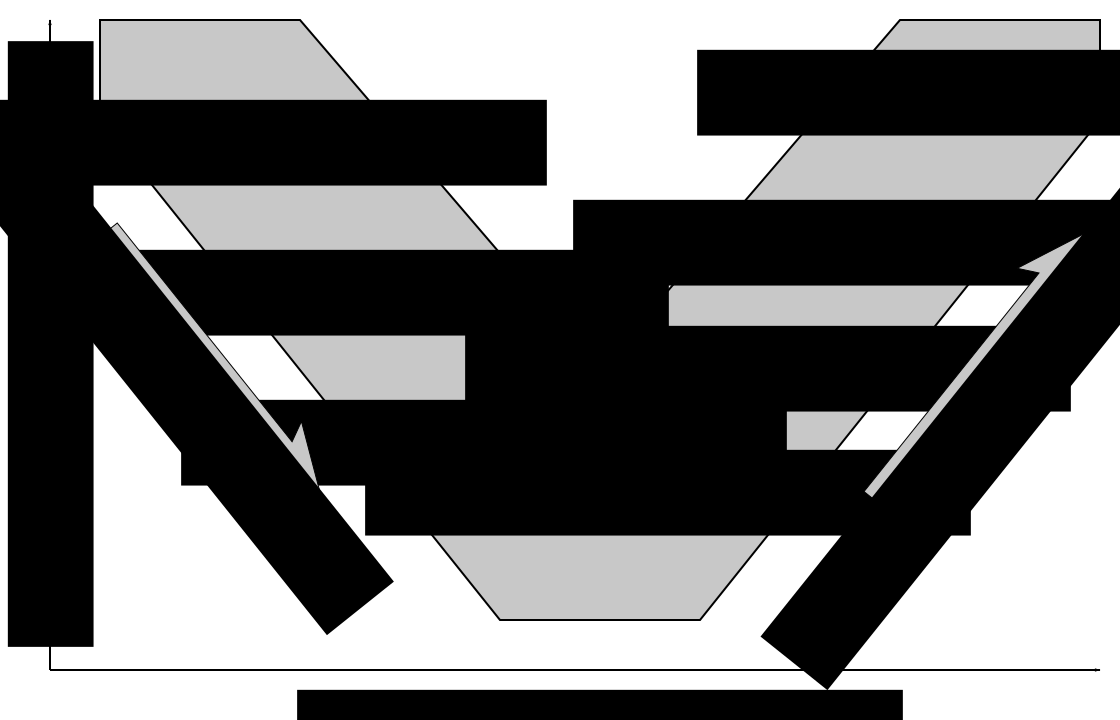
\includegraphics[width=0.5\linewidth]{1-VeeTools}%
%   \label{fig:VeeTools}
%   \caption{System Vee in the context of fuel cell systems~\cite{Forsberg1998}}
%   \label{fig:FCSystem}
% \end{figure}

% System design is not a new concept, but the tools and methods have advanced rapidly in the recent decades.  Computing power and algorithms are approaching the point where it may be possible to holistically and systematically evaluate the effects of all the design decisions that are relevant to \np{PEMFC}, \n{BOP} components, or \n{PEMFC} systems, given information about state-of-the-art component technology.  Such an evaluation tool or model could be used to optimize the \n{PEMFC}, \n{BOP} components, or \n{PEMFC} system via model-based system design for a particular application subject to preferences towards the associated cost, durability, weight, size, and other attributes.  However, as applied to \np{PEMFC} and \n{PEMFC} systems, system design is still largely based on a build-and-test approach, i.e.\ repetitively building, testing, analyzing, and redesigning prototypes to advance a concept to a final product \cite[p.~8]{DOE2007}.

% Control design inherently concerns the dynamic response of a system, as the design of a \n{FC} system often requires a compromise between transient performance and efficiency.  Thus the model's suitability depends on its ability to determine the system's dynamic response from the description of system components.

% Schmittinger and Vahidi: ``water management is of vital importance to ensure stable operation, high efficiency and to maintain the power density of \n{PEM} fuel cells in the long run'' \cite[p.~2]{Schmittinger2008}.

% The integrator is built into the simulation tool, which allows the source code to focus on the physical phenomena rather than the solution.  This also improves the robustness of the simulation, since advanced integration algorithms are available~\cite{Dassault2010}.

\section{Background}

% \section{Transport}
%
% ``Fully half of the publications in the chemical engineering journals have something to do with transport phenomena, and, in addition, there are many other disciplines where transport phenomena arise.''~\cite{Bird2004}
%
% \cite{Vasileska2006}
% \cite{Czerwinska2007}
% \cite{San1987}
% \cite{Bird2004}
% \cite{Melehy2010}
% \cite{Winter1987}
% \cite{Cercignani1988}
% \cite{Kreith2005}
% \cite{Gerber2002}
% \cite{Ajaev2012}
% \cite{Wesselingh2000}
% \cite{Bar-Meir2009}
% \cite{Koch1987}
% \cite{Tummescheit1998}
% \cite{Lauga2007}
% \cite{Bergeles2010}
% \cite{Steinmann2002}
% \cite{Boudin2008}
% \cite{Mohamed1995}
% \cite{Cantrell2008}
% \cite{Joly2008}
% \cite{Kuiken1995}
% \cite{Sherwood1984}
% \cite{Tropea2007}
%
% multiphase or multicomponent:
% \cite{Jakobsen2008}
% \cite{Kuropatenko2005}
% \cite{Boudin2011}
% \cite{Curtiss1999}
%
% specific to fuel cells:
% \cite{Anderson2010}
% \cite{Lee2009}
% \cite{McCain2007}
% \cite{Weber2004Model}
% \cite{Weber2003}
% \cite{Zhan2007}
% \cite{Shen2011}
% \cite{Commer2002}
% \cite{Karan2007}
% \cite{Kulikovsky2003}
% \cite{Meng2004}
% \cite{Zhao2011}
% \cite{Weber2006}
% \cite{Davies2009ModelicaReactionDiffusion}
% \cite{Badrinarayanan2001}


% \section{Electrochemistry}
%
% \cite{Baierlein2001}
% \cite{Bockris1956}
% \cite{Antoine2001}
% \cite{Schmickler1996}
% \cite{Wang2007}
%
% \subsection{Electro-Impedance Spectroscopy}
% \cite{Kurzweil2004}
% \cite{Yuan2009}
% \cite{Ciureanu2001}
% \cite{Makharia2005}
% \cite{Bard2001}
% \cite{Baker2005}
% \cite{Yuan2010}


% \section{Phase Change}
% \cite{Bedeaux2003}
% \cite{Garai2009}
% \cite{Ajaev2012}
% \cite{Shigeo2011}


% \section{Material Properties}
% \cite{Gilliland1936}
% \cite{Tissandier1998}
% \cite{Poling2001}
% \cite{Mason1965}
% \cite{IonPower2009}
% \cite{SGL2007}
% \cite{Din1965}
% \cite{Karim1953}
% \cite{Slattery1958}
% \cite{Venkatnathan2007}


% \section{Units}
% \cite{Rey2012}
% \cite{Allen2004}

\section{Fundamentals}

\subsection{Electrochemical Reactions}

\subsubsection{Equations}

% As in the literature (e.g.,~\cite{Bockris2000, Prentice1991}), % \cite[p. 115]{Prentice1991}
% the Tafel equation\label{mark:Tafel} can be derived from the Butler-Volmer equation under the assumption of large positive or negative overpotential.

% The Butler-Volmer equation is closely related to the Shockley diode equation~\cite{Bockris2000, Schumacher2002, Ashcroft1976}\label{mark:Shockley}. %\cite[pp.~592--595]{Ashcroft1976}
% Both electrodes and diodes involve the diffusion of charge carriers from the domain where they are a majority to where they are a minority.  The double-layer region is usually called the depletion region in semiconductors.  The Shockley equation can in fact be derived as above for the Butler-Volmer equation except that
% **concentration is fixed at the interface rather than in the bulk.
%  \begin{inparaenum}[(1)]\item there is no chemical bias ($\Delta\s{g} = 0$), \item protons are replaced by holes, \item the catalyst is the n-doped region and the ionomer is the p-doped region, \item the orientation is typically opposite such that the electric field is from the p- to the n-doped side, and \item the densities at the interface are considered to be dependent on the carrier densities in the middle of the minority regions (which are determined by the doping levels) rather than vice versa\end{inparaenum}.  It follows from the last point that the densities $\s{rho}_\text{a}$ and $\s{rho}_\text{b}$ in \autoref{eq:ExchangeCurrentDensity} are the minority densities rather than the densities at the interface (which are essentially the majority densities).  Also as a result, the entire electric field is applied to one exponential.
% \begin{equation}
%   \label{eq:Shockley}
%   \s{z}\s{J} = \s{J}[^o]\group{e^{\s{Pe}} - 1}
% \end{equation}
% which is the Shockley diode equation where $\s{Pe} = \s{w}/\s{T}$.

\section{Implementation}

\subsection{Connectors}

% ``Connectors and connector designs are crucial for the modular modeling of complex physical systems.''~\cite{Franke2009}

% For each effort\slash{}flow pair, exactly one equation must be added to a model.

% The instantaneous material current is zero since particles are discrete (the event when a particle crosses a surface is instantaneous), so current is averaged over time.

% **\cite[p.~395]{Fritzson2004}
% ``As in all system design, defining the interfaces between the components of a system model is one of the most important design tasks since this lays the foundation for the communication between the components, thereby also heavily influencing the decomposition of the model.''

\section{RelatedTheory}
\subsection{Hertz-Knudsen Equation}
\label{sec:HertzKnudsen}

The model can be related to the Hertz-Knudsen equation, which describes the rate of phase change between a

% The Hertz-Knudsen equation describes the rate of phase change...**

Since it is difficult to quantify the diffusion length~\s{L}, we will write it as a number of mean free paths of an ideal gas at the same conditions.  That number is the reciprocal of the Knudsen number; therefore, the reciprocal of length is replaced by the Knudsen number divided by the mean free path of an ideal gas ($1/\s{L} = \sqrt{2}\timessep\pi\timessep\s{d}^2\timessep\s{q}\timessep\s{rho}\timessep\s{Kn}$)~\cite{Cussler1997}.
\begin{equation}
  \dot{N} = \sqrt{2}\timessep\pi\timessep\s{d}^2\timessep\s{q}\timessep\s{rho}\timessep\s{Kn}\timessep\s{k}\timessep\s{A}\timessep\group{\frac{\s{rho}[_g]}{\s{eta}[_g]} - \frac{\s{rho}\sub{_g}[_c]}{\s{eta}\sub{_g}[_c]}}
\end{equation}

The first equation (\ref{eq:PhaseChange4}) is closely related to the Hertz-Knudsen equation.  If we assume that the material resistivity is equal to the estimate from kinetic theory (\autoref{eq:MaterialResistivity}),
\begin{equation}
  \dot{N} = \frac{2\s{k}\s{A}}{3\pi\s{d}^2\s{q}}\sqrt{\frac{1}{\pi\s{m}}}\group{\frac{\sqrt{\s{T}[_g]}}{\s{L}[_g]} - \frac{\sqrt{\s{T}\sub{_g}[_c]}}{\s{L}\sub{_g}[_c]}}
\end{equation}
Writing each length in terms of the Knudsen number ($1/\s{L} = \sqrt{2}\pi\timessep\s{d}^2\timessep\s{q}\timessep\s{rho}\timessep\s{Kn}$, since the gas is ideal~\cite{Cussler1997}),
%[p. 177]; matches \url{http://en.wikipedia.org/wiki/Knudsen_number}
\begin{equation}
  \dot{N} = \frac{2\s{k}\s{A}}{3}\sqrt{\frac{2}{\pi\s{m}}}\group{\s{Kn}[_g]\s{rho}[_g]\sqrt{\s{T}[_g]} - \s{Kn}\sub{_g}[_c]\s{rho}\sub{_g}[_c]\sqrt{\s{T}\sub{_g}[_c]}}
\end{equation}
If the area factor~(\s{k}) is $3/4$. % **justify
\begin{equation}
  \dot{N} = \frac{\s{A}}{\sqrt{2\pi\s{m}}}\group{\s{Kn}[_g]\s{rho}[_g]\sqrt{\s{T}[_g]} - \s{Kn}\sub{_g}[_c]\s{rho}\sub{_g}[_c]\sqrt{\s{T}\sub{_g}[_c]}}
\end{equation}
If the Knudsen numbers are unity,
\begin{equation}
  \label{eq:HK}
  \dot{N} = \frac{\s{A}}{\sqrt{2\pi\s{m}}}\group{\s{rho}[_g]\sqrt{\s{T}[_g]} - \s{rho}\sub{_g}[_c]\sqrt{\s{T}\sub{_g}[_c]}}
\end{equation}
which is the Hertz-Knudsen equation~\cite{Ytrehus1997}.  Otherwise since the gas is ideal,
\begin{equation}
  \dot{N} = \frac{\s{A}}{\sqrt{2\pi\s{m}}}\group{\frac{\s{Kn}[_g]\s{p}[_g]}{\sqrt{\s{T}[_g]}} - \frac{\s{Kn}\sub{_g}[_c]\s{p}\sub{_g}[_c]}{\sqrt{\s{T}\sub{_g}[_c]}}}
\end{equation}
which is the Hertz-Knudsen-Langmuir equation~\cite{Frohn2000} with \s{Kn}[_g] as the condensation coefficient and $\s{Kn}\sub{_g}[_c]$ as the evaporation coefficient.

% Arguments against Hertz-Knudsen-Langmuir

%\section{Linear Circuits and Electromagnetism}

%\subsection{Capacitance}

% A capacitor can be viewed as a concentration cell, i.e., a device that allows properties to be stored and released from a nonuniform state.

% \begin{equation}
%   \label{eq:Capacitor}
%   \s{I} = \s{C}\diff{\s{w}}{\s{t}}
% \end{equation}

% \cite[p.~307]{Thomas1998}

%\subsection{Inductance}

% \begin{equation}
%   \label{eq:Inductor}
%   \s{w} = \s{L}\diff{\s{zI}}{\s{t}}
% \end{equation}

% \cite[p.~315]{Thomas1998}

%\subsection{Maxwell Equations}

% \begin{subequations}
%   \begin{align}
%     \label{eq:Maxwell}
%     &\oint\vec{\s{E}}\cdot d\vec{\s{A}} = \frac{\s{Q}[_encl]}{\s{epsilon}[_0]}\\
%     &\oint\vec{\s{B}}\cdot d\vec{\s{A}} = 0\\
%     &\oint\vec{\s{D}}\cdot d\vec{\s{L}} = \s{mu}[_0]\group{\s{I}[_c] + \s{epsilon}[_0]\diff{\s{Phi}[_E]}{\s{t}}}\\
%     &\oint\vec{\s{E}}\cdot d\vec{\s{L}} = \s{mu}[_0]\group{-\diff{\s{Phi}[_B]}{\s{t}}}
%   \end{align}
% \end{subequations}

% \cite[p. 959]{Young1996}

% Electrons (or ions) traveling in parallel pull together (e.g., Ampere's law), but like charges spread apart (e.g., Coulomb's law).

% \url{http://en.wikipedia.org/wiki/Ampere-meter}:
%   ``Einstein proved that a magnetic field is the relativistic part of an electric field.  This means that while an electric field acts between charges, a magnetic field acts between moving charges (as a charge moves through space more quickly and through time more slowly, its electromagnetic force becomes more magnetic and less electric).  Therefore, the pole strength is the product of charge and velocity.''

% Other possibly related theories:
%   Reduced mass
%     Follows from exchange or transport resistances in series or parallel?  Should the exchange resistances be in parallel?
%   Thermal noise
%    ~\cite{Sarpeshkar1993}
%   Stefan problems
%   Kelvin equation
%   2nd law of thermodynamics (and 3rd?)
%     Make analogy to control system; closed physical systems are always damped.
%   Morse potential
%   Arrhenius equation
%     \cite[pp.~529--530]{Brown2000}
%   Nernst-Einstein equation
%     \url{http://alford.bios.uic.edu/teaching/Nernst.html}
%     Discussion in~\cite{Weber-ChemRev2004}
%   Transport in dilute solutions due to migration in an electric field
%     \cite[Equation~11.1, p.~241]{Newman1991}, \cite[p.~325]{Newman1991}, \cite[Equation~16, p.~333]{Newman1991}
%   Nernst-Planck equation
%     Discussion in~\cite{Weber-ChemRev2004}
%   Concentrated solution theory
%     Discussion in~\cite{Weber-ChemRev2004}
%   Dilute solution theory
%     Discussion in~\cite{Weber-ChemRev2004}
%   Speed of sound
%   Non-equilibrium thermodynamics
%   Thermoelectrics (p.~0 and p.~1 of 8/8/11 notes)
%   Einstein-Stokes equation
%   Maxwell-Boltzmann statistics
%     \url{http://en.wikipedia.org/wiki/Boltzmann_statistics}
%   Poisson's equation
%   Full set of semiconductor equations
%     \url{http://www.iue.tuwien.ac.at/phd/entner/node9.html}
%   Hertz-Knudsen equation
%   Langmuir equation
%     \url{http://en.wikipedia.org/wiki/Langmuir_equation}
%   Fermi gas
%     \url{http://www.physics.thetangentbundle.net/wiki/Statistical_mechanics/Fermi_gas}
%   Fermi energy
%   Cauchy equation, \cite[p.~80]{Bird2002}
%   Cellular automata
%   Equimolar counter-diffusion
%   Ultrarelativistic fluid (if possible; see 10/3/11 notes)
%     \url{http://en.wikipedia.org/wiki/Ultrarelativistic_fluid}
%   Relate the use of hyperbolic tangent in the model to
%     \url{http://en.wikipedia.org/wiki/Velocity-addition_formula} and Lorentz transformation.
%   Explain relation of velocity and Gibbs energy difference and electrical potential difference.
%   Boltzmann distribution \cite[p.~460]{Deen1998}
%   Boltzmann equation
%   Lattice Boltzmann
%   Shell momentum balance
%     \url{http://en.wikipedia.org/wiki/Shell_balance}
%     \url{http://www.syvum.com/cgi/online/serve.cgi/eng/fluid/fluid_2a.html}
%   Stokes law
%     \url{http://en.wikipedia.org/wiki/Stokes%27_law_(sound_attenuation)}
%   Bernoulli's principle
%   Electrochemical potential of electrons
%     \cite[pp.~254--256]{Ashcroft1976}
%   Wiedemann-Franz law
%   Stoke's theorem (12/15/12 p. 2 and Wikipedia Einstein relation)

\section{Cell}
\subsection{Linearization}
%**Linearize the cell at various electrical load points.

% The model linearization gives the values of the \s{A}, \s{B}, \s{C}, and \s{D} matrices of the state space representation:
% \begin{subequations}%
%   \begin{align}%
%     \dot{x} &= \s{A}\times\s{x} + \s{B}\times\s{u}\\
%     \s{y} &= \s{C}\times\s{x} + \s{D}\times\s{u}
%   \end{align}
%   \label{eq:StateSpace}%
% \end{subequations}

% \caption[FC response in the frequency domain with a sinusoidal load]{FC response in the frequency domain with a sinusoidal load: \subref{fig:FCExp-Sim-10a} Bode diagram of the electrochemical impedance of the linearized \n{FC} and \subref{fig:FCExp-Sim-10b} thermodynamic efficiency of the \n{FC} in the complex plane}%**Add plots.

% **Use this paper to validate the model under step load change:~\cite{Wang2006}.

% The HNEI pol curves involve decreasing current, which results in the overshoot in voltage.

% \caption[FC response in the time domain with a sinusoidal load]{FC response with a sinusoidal load: \subref{fig:FCExp-Sim-9a} losses due to resistance, activation, and concentration in the \n{PEM}, GDL, and catalyst layers and \subref{fig:FCExp-Sim-9b} cathode catalyst layer temperature and \n{PEM} hydration}

% \autoref{fig:FCExp-Sim-10} illustrates the same dynamics as \autoref{fig:FCExp-Sim-9}, but in the frequency domain.  The baseline model is linearized with  varying reactant humidity levels about a quiescent load of \SI{0.75}{A/cm^2}.  The transfer function of $V(s)/I(s)$% **Add symbols.
%  is evaluated from the state-space representation. \autoref{fig:FCExp-Sim-10a} shows the response in a Bode plot, which has Cartesian coordinates of magnitude and angle vs.\ frequency. \autoref{fig:FCExp-Sim-10b} shows the thermodynamic efficiency of the cell in the complex plane.  The cell is most efficient where the real part of the efficiency is **.
% **Rerun with  varying reactant humidity, update the figures, and comment further.
% **Plot efficiency instead of EMF.
% **Add to nomenclature: $\eta$ & Thermodynamic efficiency.

\subsection{Results and Discussion}

\begin{figure}[htbp]
  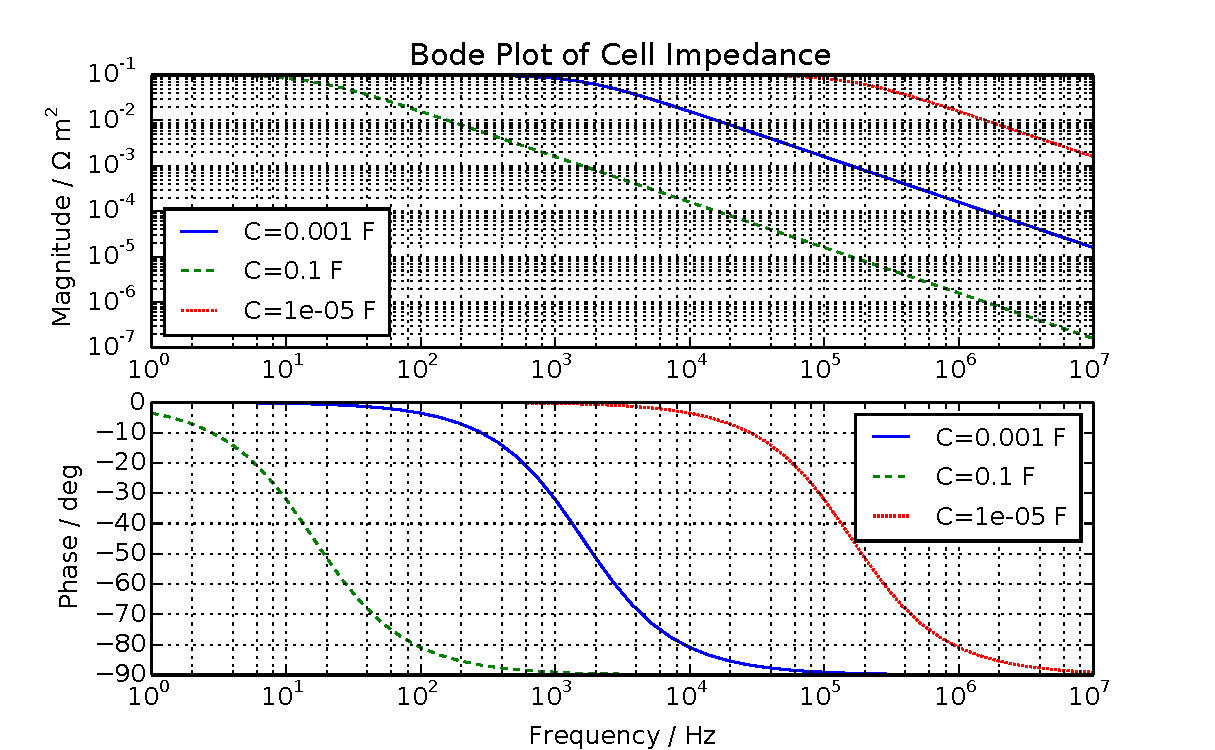
\includegraphics[width=\linewidth]{Results/Cell/Model/Linearization/Bode}%
  \caption{}%
  \label{fig:}
\end{figure}

\begin{figure}[htbp]
  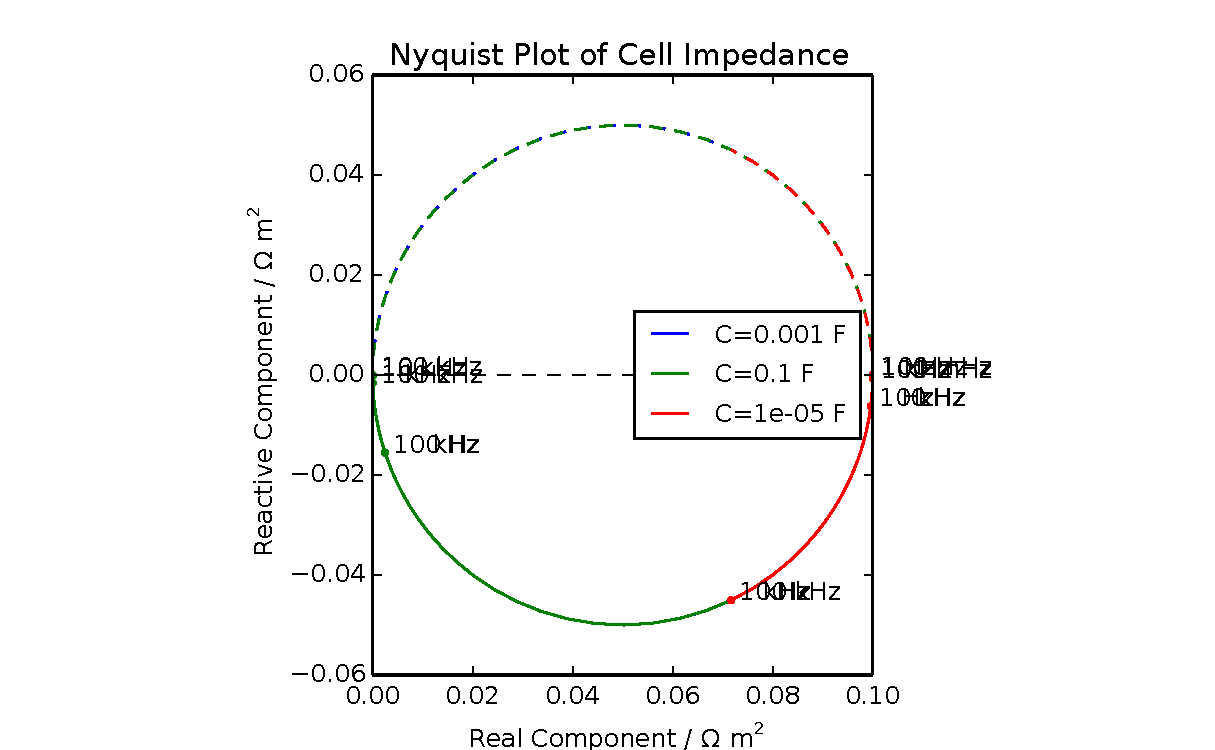
\includegraphics[width=\linewidth]{Results/Cell/Model/Linearization/Nyquist}%
  \caption{}%
  \label{fig:}
\end{figure}

% \begin{figure}[htbp]
  % \includegraphics[width=0.5\linewidth]{FCDesc-EISBodeMarkup}% \caption[Bode
  % plot of the impedance of a \n{PEMFC}]{Bode plot of the impedance of a \n{PEMFC}
  % \input{../Dissertation/Figures/FCDesc-EISBodeMarkup}}%
  % \label{fig:FCDesc-EISBode} 
% \end{figure}%

**compare to~\cite{Franco2007}

% \cite{Kurzweil2004}: ``Simply speaking, every phase boundary causes its own arc in the complex plane''

% Randles cell does not include inductance.

% \autoref{fig:FCDesc-EISBode} shows that there are two resonances in the \n{PEMFC} response due to transport phenomena.

% \begin{figure}[htbp] \includegraphics[width=8cm]{FCDesc-EISBode}%
  % \caption[Bode plot of the impedance of a \n{PEMFC}]{Bode plot of the impedance of
  % a \n{PEMFC} \input{../Dissertation/Figures/FCDesc-EISBode}}
% \end{figure}%

% Nyquist plot: Plot of a transfer function in the Gaussian number plane over varying frequencies (also Cole-Cole plot or complex impedance diagram \cite[p. 141]{Yuan2009})

\subsubsection{Water}

% According to a review by Schmittinger and Vahidi, poor water management is one of the three main factors in short life and degradation of \np{PEMFC} \cite[p.~1]{Schmittinger2008}.

\section{Performance}

% \autoref{tab:Performance} gives information regarding the complexity of the models and the time to compile and simulate them.  The columns correspond to the first list in \autoref{sec:PerformanceMetrics}.
\autoref{tab:SegmentedStatistics} gives information regarding the complexity of the models and the time to compile and simulate them.  There were no nonlinear systems of equations after manipulation and no numerical Jacobians for any of the models.  All of the states were statically selected (i.e., no dynamic state selection).
% % **Verify all this.

% **translation time is rounded down to the second

% \begin{landscape}
%   \begin{table}[hbt]
%     \caption{Complexity of the models and the time to compile and simulate}%
%     \label{tab:Performance}
%     \begin{contextbox}
  Modeling and simulation statistics:
  \begin{itemize}
    \item Number of variables: 31990
    \item Number of time-varying variables: 12711
    \item Number of states: 266
    \item Sizes of the nonlinear systems of equations: None
    \item Translation time: \SI{69}{s}
    \item Simulation time: \SI{11.3}{s}
  \end{itemize}
\end{contextbox}
%   \end{table}
% \end{landscape}
 
% \begin{landscape}
%   \begin{table}[hbt]
%     \caption{Statistics on the segmented cell model and its simulation}%
%     \label{tab:SegmentedStatistics}
%       \begin{tabular}{cccccccc}
  \toprule
  \textbf{Number of}  & \textbf{Number of} & \textbf{Number of time-} & \textbf{Number of} & \textbf{Number of} & \textbf{Size of largest} & \textbf{Translation} & \textbf{Simulation} \\
  \textbf{segments} & \textbf{variables} & \textbf{varying variables} & \textbf{states} & \textbf{linear systems} & \textbf{linear system} & \textbf{time / s} & \textbf{time / s} \\
  \midrule
  1 & 23953 & 6224 & 266 & 674 & 8 & 130 & 13.7 \\
  2 & 23957 & 6222 & 266 & 672 & 8 & 133 & 16.1 \\
  \bottomrule
\end{tabular}
%   \end{table}
% \end{landscape}

% \autoref{fig:VariablesCompilation} shows a scatter plot of the time to compile the model versus the number of variables.  \autoref{fig:Variables} shows a scatter plot of the total simulation time versus the number of variables.  \autoref{fig:VaryingVariables} shows a scatter plot of the total simulation time versus the number of time-varying variables.  \autoref{fig:States} shows a scatter plot of the total simulation time versus the number of states.  \autoref{fig:Sizes} shows a scatter plot of the total simulation time versus the sum of the cubes of the sizes of the linear systems of equations.
% from Chris:  the computational complexity of solving a set of linear equations numerically is O(n^3) -- all the common algorithms have the same order (LU decomposition, Gauss elimination,...).  The only difference is for iterative solutions of sparse matrix problems, but those are not used in Dymola.

% \begin{figure}[htbp]
%   \includegraphics[width=\linewidth]{Results/Cell/Model/Performance/VariablesCompilation}%
%   \caption{Compilation time vs.\ number of variables}%
%   \label{fig:VariablesCompilation}
% \end{figure}

% \begin{figure}[htbp]
%   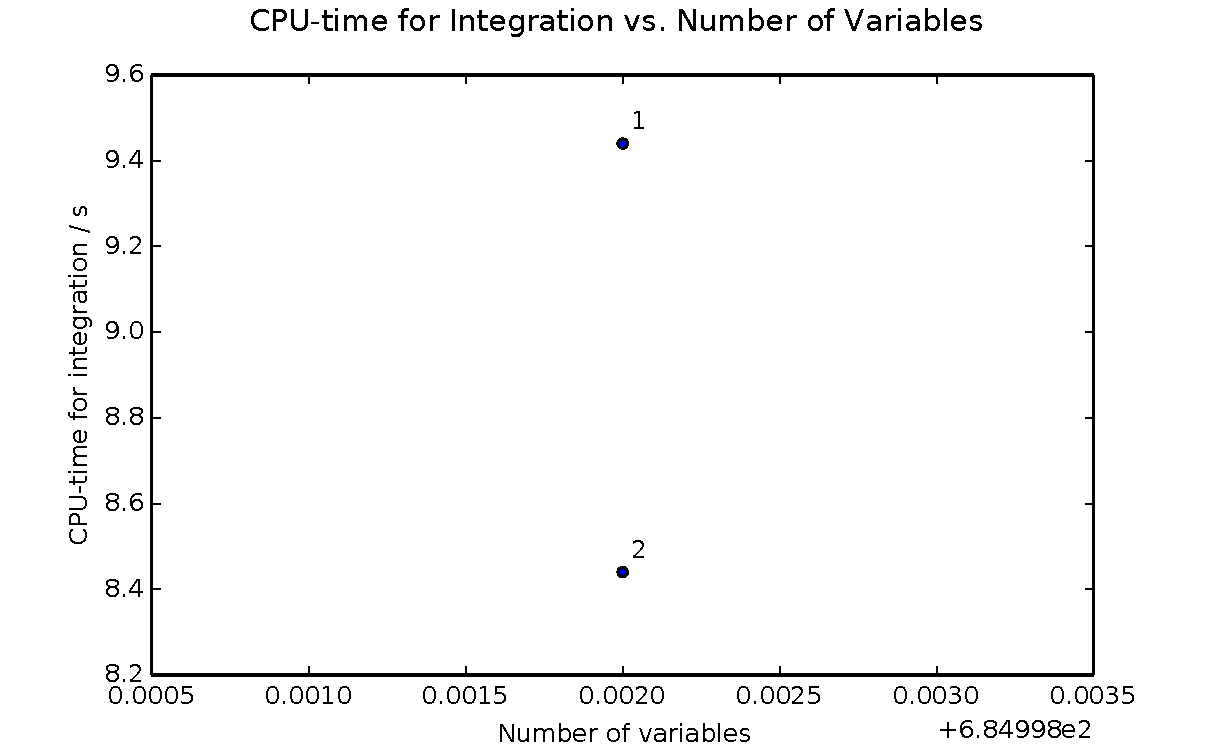
\includegraphics[width=\linewidth]{Results/Cell/Model/Performance/Variables}%
%   \caption{Simulation time vs.\ number of variables}%
%   \label{fig:Variables}
% \end{figure}
% 
% \begin{figure}[htbp]
%   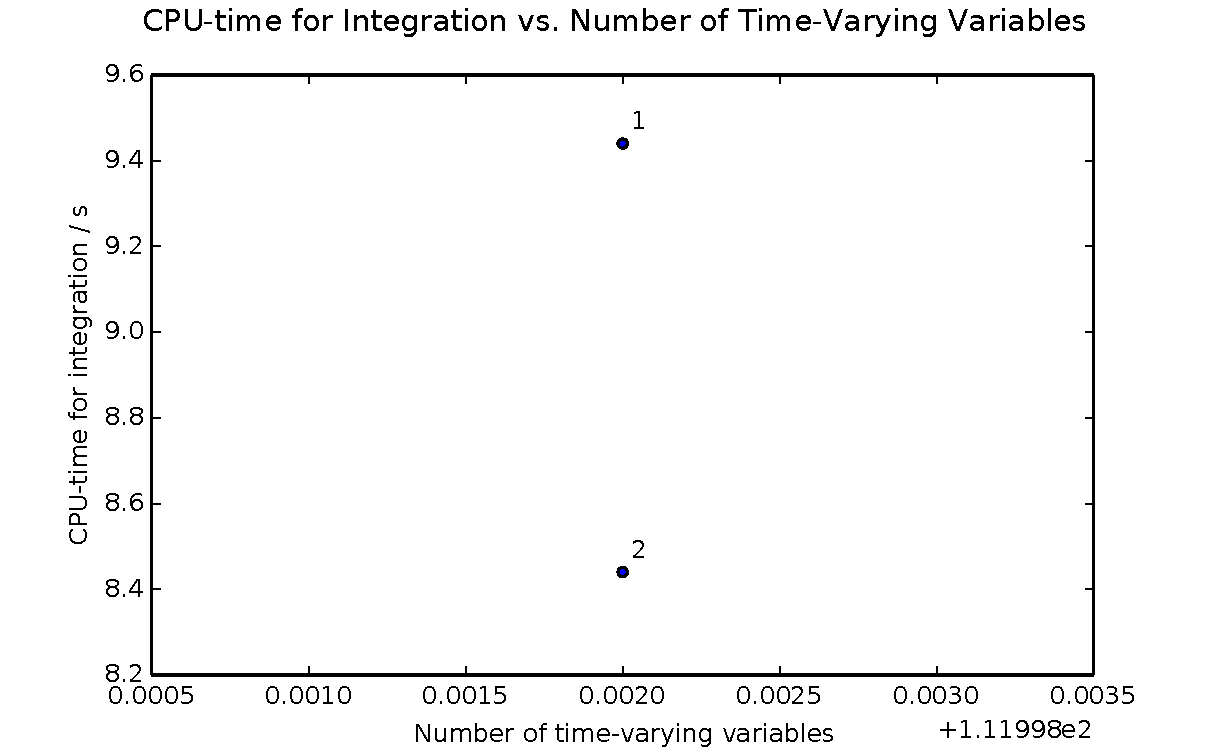
\includegraphics[width=\linewidth]{Results/Cell/Model/Performance/VaryingVariables}%
%   \caption{Simulation time vs.\ number of time-varying variables}%
%   \label{fig:VaryingVariables}
% \end{figure}
% 
% \begin{figure}[htbp]
%   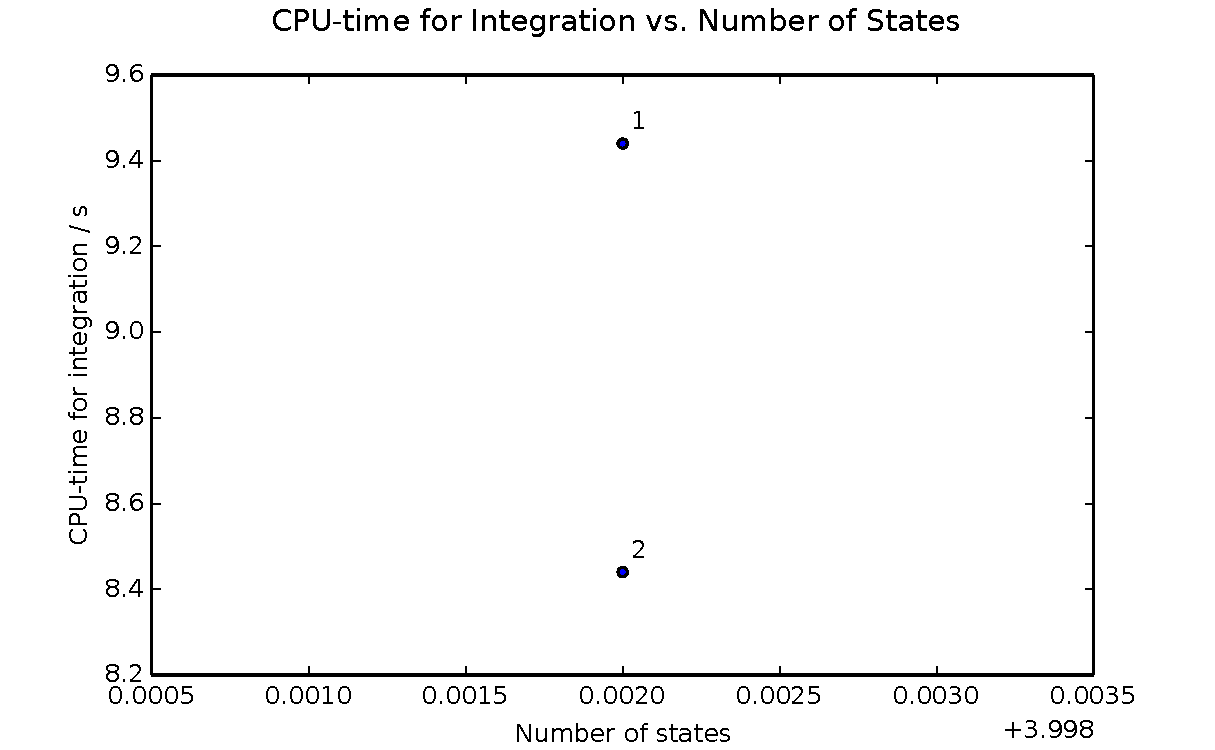
\includegraphics[width=\linewidth]{Results/Cell/Model/Performance/States}%
%   \caption{Simulation time vs.\ number of states}%
%   \label{fig:States}
% \end{figure}
% 
% \begin{figure}[htbp]
%   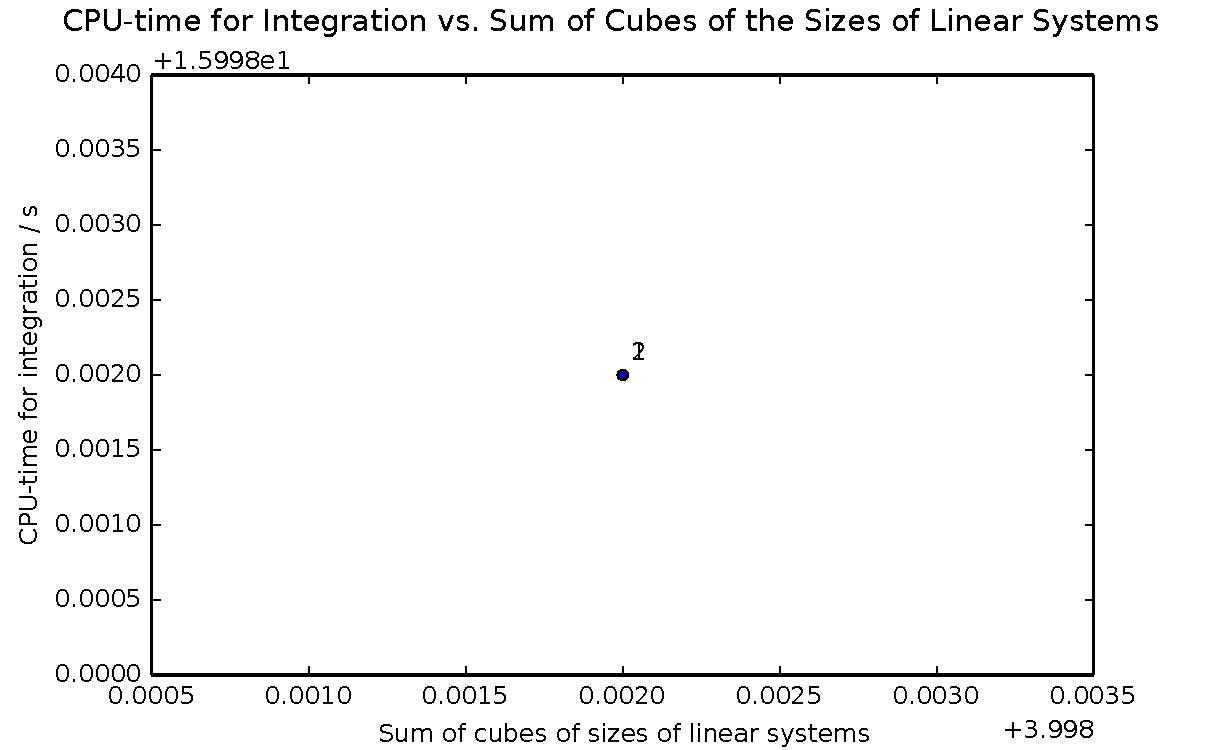
\includegraphics[width=\linewidth]{Results/Cell/Model/Performance/Sizes}%
%   \caption{Simulation time vs.\ sum of cubes of the sizes of the linear systems}%
%   \label{fig:Sizes}
% \end{figure}

% \autoref{fig:CPUtimes} shows a plot of CPU time for several of the simulations. **Discuss.

% \begin{figure}[htbp]
%   \includegraphics[width=\linewidth]{Results/Cell/Model/CPUtime/CPUtimes}%
%   \caption{Simulation time as a function of real time for several polarization simulations}%
%   \label{fig:CPUtimes}
% \end{figure}

% \autoref{tab:DominateError} lists information about the top ten states that limited the simulation speed.  The data is for the baseline simulation.  According to the Dymola 7.4 user's manual, \emph{limit stepsize} is the number of times that the ``error in the component [\ldots]\ exceeded the tolerance and forced the integrator to reduce the step size''.  \emph{Dominate error} is the number of times that the ``component [\ldots]\ dominated the error estimate.''  \emph{Exceeds 10\% of error} is the number of times that the ``error contribution from the component [\ldots]\ exceeded 10 \% of the total error estimate''~\cite{Dassault2010}.
% **Discuss

% \begin{table}[hbt]
%   \caption{Critical states with respect to simulation speed}%
%   \label{tab:DominateError}
%   \begin{tabular}{ccccl}
%     \toprule
%      & \textbf{Limit} & \textbf{Dominate} & \textbf{Exceeds} & \\
%     \textbf{Rank} & \textbf{stepsize} & \textbf{error} & \textbf{10\% of error} & \textbf{Component} \\
%     \midrule
%     1 & 0 & 13 & 45 & \modelica{CriticalDamping.x[1]} \\
%     2 & 0 & 29 & 47 & \modelica{CriticalDamping.x[2]} \\
%     3 & 0 & 9 & 48 & \modelica{CriticalDamping.x[3]} \\
%     4 & 0 & 0 & 23 & \modelica{Bessel.x[1]} \\
%     5 & 0 & 3 & 53 & \modelica{Bessel.x[2]} \\
%     6 & 0 & 2 & 47 & \modelica{Bessel.x[3]} \\
%     7 & 0 & 0 & 7 & \modelica{Butterworth.x[1]} \\
%     8 & 0 & 5 & 36 & \modelica{Butterworth.x[2]} \\
%     9 & 0 & 0 & 31 & \modelica{Butterworth.x[3]} \\
%     10 & 0 & 15 & 26 & \modelica{ChebyshevI.x[2]} \\
%     \bottomrule
%   \end{tabular}
% \end{table}
% % From ``Results/Cell/Model/dominate states.xls''

\section{Concluding Remarks}

The model implementation is highly modular and reconfigurable.  It uses advanced features of the Modelica~\cite{Modelica3.3} language, including:
\begin{itemize*}
  \item Expandable bus connectors
  \begin{itemize*}
    \item For species within phases or phase change interactions
    \item For phases within boundaries
  \end{itemize*}
  \item Stream connectors
  \begin{itemize*}
    \item For the purely advective flows of chemical reactions and phase change
  \end{itemize*}
  \item Replaceable and conditional models, functions, connectors, and variables
  \begin{itemize*}
    \item To provide flexible choices for the included species and the modeling assumptions
    \item To eliminate unnecessary overhead
  \end{itemize*}
  \item Multi-dimensional arrays with variable sizes
  \begin{itemize*}
    \item To allow flexible choices for the included boundaries and the components of translational momentum
  \end{itemize*}
  \item Custom physical connectors that utilize generalized Kirchhoff circuit laws in unique ways
  \begin{itemize*}
    \item For Amagat's law of additive volumes
    \item For Dalton's law of additive pressures
    \item For chemical stoichiometry and equilibrium
  \end{itemize*}
  \item Instantiation
  \begin{itemize*}
    \item To represent the physical hierarchy: species within phases within subregions within regions within assemblies
  \end{itemize*}
  \item Inheritance to represent specialized versions of classes, e.g.,
  \begin{itemize*}
    \item Carbon is an incompressible species
    \item An incompressible species is a general species with special assumptions
  \end{itemize*}
\end{itemize*}

The hypothesis is that \n{FC} models can be improved and this will simplify the task of \n{FC} system design and enable more reliable, robust, and well-integrated systems.
For instance, consider the redesign of hardware (e.g., flow plate geometry, manifolding, and choice of humidifier(s)) and controls (e.g., sensors, actuators, and control algorithms) for a \n{FC} system in order to improve dynamic response.
Currently, different tools are required to analyze hardware design and control design, and as a result, the hardware is typically designed before the controls, although the two areas are highly coupled and both have a strong impact on dynamics.
If a modeling tool could evaluate modifications to both hardware and controls, engineers could achieve a more optimal and synergistic design by simultaneously optimizing hardware and controls.

For example, adding a cathode exit valve will allow cathode pressure (and thus peak \n{FC} power) to be dynamically controlled, but will require additional hardware (with increases in mass, volume, cost, and complexity) and the higher pressures will come at the price of increased compressor or blower power.  As another example, some hardware designs may allow \n{FC} hydration and temperature to be passively instead of actively controlled, but their use may reduce the robustness of the system to operating conditions.

``Definitions of causality and nonanticipation suffer from the post hoc ergo propter hoc (it happened before, hence it caused) fallacy.''~\cite{Willems - The Behavioral Approach to Open and Interconnected Systems}

Spatially, the proposed model does not couple the states of geometrically separate regions.  They are only coupled through time derivatives.  So the systems of equations are not nearly as large as for \n{CFD} approaches.

**even though the upstream discretization scheme has only been implemented between two connectors, it is general and can be applied to higher-order connections.

**A differential version of the model itself can be used to determine the adjustment factors that allow the model to be used at a higher level of discretization (e.g., pipe flow, thermal convection, and electrochemical reaction ****confirm).  I.e., the model is self-consistent.

% It is challenging to develop declarative models of chemical\slash{}fluid\slash{}thermal systems.  Much work remains to be done.  Even though there are model libraries such as \modelica{Modelica.Fluid}, Cellier's comments from twenty years ago~\cite{Cellier1991} are still relevant:
% \begin{quote}
%   Electrical circuits are so well understood that it is possible to use a model to design an overall circuit in all likelihood it will work just as predicted by the model.  This is also true for some mechanical systems [\dots].  This is no longer true for chemical systems.  Many factors influence a chemical reaction, factors which are all of approximately equal importance.  Therefore, models that are valid for a large set of experiments cannot be specified.
% \end{quote}
% [\dots]
% \begin{quote}
%   It is unclear how we can design a systematic methodology, a generalized bond graph maybe, that ensures conservation of both energy and mass simultaneously.  Such an investigation might therefore be a fruitful topic for another Ph.D. dissertation---not exactly an easy task either.
% \end{quote}

``Since the convection problems are primarily influenced by the associated flow field, the solution of convection problems starts with the solution of the flow field governed by the conservation laws of mass and momentum equations such as the Navier-Stokes equations, followed by a solution of energy or mass concentration equations.  These governing equations constitute a set of coupled nonlinear partial differential equations for three velocity components, pressure, temperature [Background.tex] or mass concentration.  Major computational difficulties arise due to the presence of nonlinear convective terms as well as for [the] pressure term for which there is no distinct equation.''\cite{Majumdar2005}